\documentclass{beamer}

\usepackage[utf8]{inputenc}
\usepackage{hyperref}
\usepackage{times}
\usepackage{graphicx}
\usepackage[english]{babel}
%\usepackage[onehalfspacing]{setspace}
\usepackage{amsmath}
\setbeamertemplate{section in toc}[sections numbered]
\setbeamertemplate{subsection in toc}[subsections numbered]
\usepackage{bm}


%Information to be included in the title page:
\title{Guided Diffuison Quantum Monte Carlo for Calculating Zero Point Energies}
\author{Simon Neidhart}
\institute{Department of Physics, University of Basel}
\date{\today}


\begin{document}
\frame{\titlepage}

\begin{frame}
\frametitle{Table of Contents}
\tableofcontents
\end{frame}

\section{Introduction}
\begin{frame}
\frametitle{Introduction}
\begin{itemize}
\item DQMC solves the Schrödinger equation and gives the quantum-mechanical ground state energy to then calculate the zero point energy (ZPE).
\item A Gaussian guiding wave function is used to improve the performance.
\item DFTB+ is used for calculation the energy.\cite{dftbp}
\end{itemize}
\end{frame}

\section{The DQMC Algorithm}
\begin{frame}
\frametitle{The Unguided DQMC Algorithm \cite{mccoy}}
\begin{itemize}
\item The stationary solution of the diffusion equation satisfies the Schrödinger equation and has the propagator $G(\bm{x},\bm{y};\Delta t) = \frac{1}{\sqrt{2 \pi \Delta t}} e^{-(\bm{x}-\bm{y})^2/(2\Delta t)} e^{-\Delta t (V(\bm{y}) - E_T)}$.
\item We simulate a ensemble of walkers to reach this stationary solution and the Schrödinger equation is solved.
\item The propagator consists of a diffusion term $\frac{1}{\sqrt{2 \pi \Delta t}} e^{-(\bm{x}-\bm{y})^2/(2\Delta t)}$ and a branching term $e^{-\Delta t (V(\bm{y}) - E_T)}$.
\item The diffusion term is simulated by randomly displacing the walker from its previous position according to a Gaussian distribution.
\item The branching term updates the weight of a walkers according to which the walker survives, reproduces or dies.
\item The trial energy $E_T$ is then adjusted to keep the population of walkers stable.
\item With time, the trial energy $E_T$ converges.
\end{itemize}
\end{frame}

\section{The Guiding Wave Function}
\begin{frame}
\frametitle{The Guiding Wave Function \cite{cyrus}}
\begin{itemize}
\item Harmonic approximation of the potential energy surface with the Hessian matrix.
\item Gaussian guiding wave functions along the normal modes $\psi_T(x) = \mathcal{N} e^{-x^2/(2 \sigma^2)}$.
\item The width of the Gaussian is given by $\sigma^2 = \frac{1}{\omega m}$, where $\omega^2$ is the corresponding eigenvalue of the Hessian matrix.
\item This is incorporated to the algorithm with a drift velocity $\bm{v}(\bm{x}) = \nabla_{\bm{x}} \psi_T(\bm{x})$ which is added to the pure diffusion and a kinetic energy term in the local energy $E_L(\bm{x}) = (H\psi_T(\bm{x}))/\psi_T(\bm{x})$ which replaces the potential energy in the branching step.

\end{itemize} 

\end{frame}

\begin{frame}
\frametitle{The Guiding Wave Function}
\begin{center}
\scalebox{0.35}{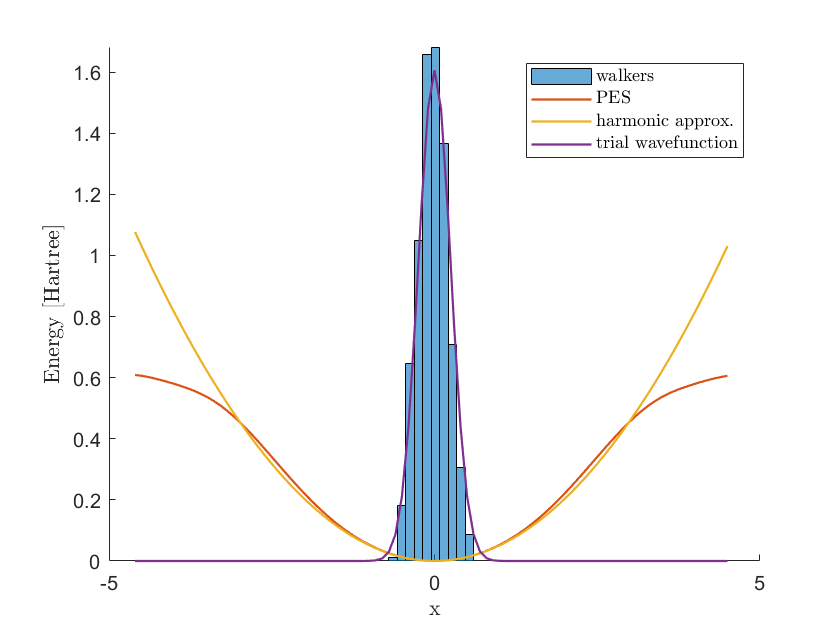
\includegraphics{trialwf.png}}\\
Fig. 1. Typical dimension in the coordinate system of the normal modes.
\end{center}

\end{frame}

\section{Input and Output}
\begin{frame}
\frametitle{Input and Output}
Input:\\
\begin{itemize}
\item Equilibrium geometry of the atoms (must not be perfectly accurate as geomety will be optimized by DFTB+ in the beginning)
\item Masses of the atoms
\end{itemize}
Output:
\begin{itemize}
\item Zero point energy
\item Walker positions give a sample of the nucleonic wave function
\end{itemize}
\end{frame}

\section{Results}

\subsection{$C_2 H_6$}
\begin{frame}
\frametitle{Results}
\framesubtitle{$C_2 H_6$ (first test case)}
\begin{center}
\scalebox{0.20}{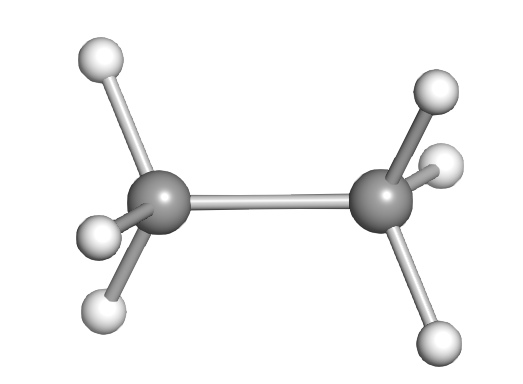
\includegraphics{p1.png}}\\
Fig. 2. Input structure of Ethane
\end{center}
First test case to develop the algorithm and check the result with a literature value.
\end{frame}

\begin{frame}
\frametitle{Results}
\framesubtitle{$C_2 H_6$ (first test case)}
Simulation with 1000 walkers for 2000 time steps
\begin{center}
\scalebox{0.25}{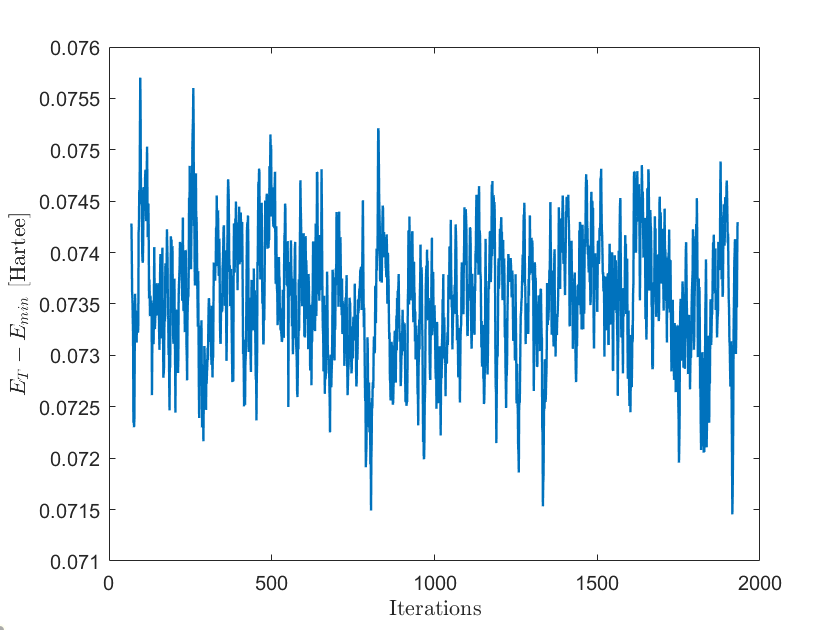
\includegraphics{fig1.png}}\\
Fig. 3. Fluctuation of the ZPE after equilibration.
\end{center}
ZPE = 0.07356 hartee with a standard deviation of 0.00060 hartee. The literature value is 0.073927 hartree \cite{c2h6}.\\

\end{frame}

\begin{frame}
\frametitle{Results}
\framesubtitle{$C_2 H_6$ (first test case)}
Simulation with 1000 walkers for 2000 time steps
\begin{center}
\scalebox{0.25}{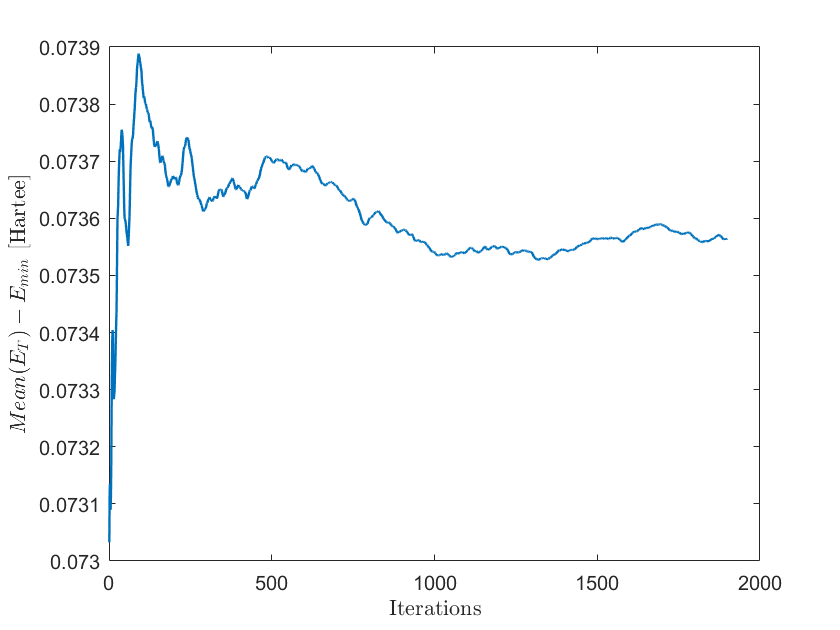
\includegraphics{fig2.png}}\\
Fig. 4. Convergence of the ZPE after equilibration.
\end{center}
Simulation time: 14 hours. $\approx$ 0.02 seconds per energy calculation.

\end{frame}

\subsection{$C_{12} H_{10} O$}

\begin{frame}
\frametitle{Results}
\framesubtitle{$C_{12} H_{10} O$}
\begin{center}
\scalebox{0.20}{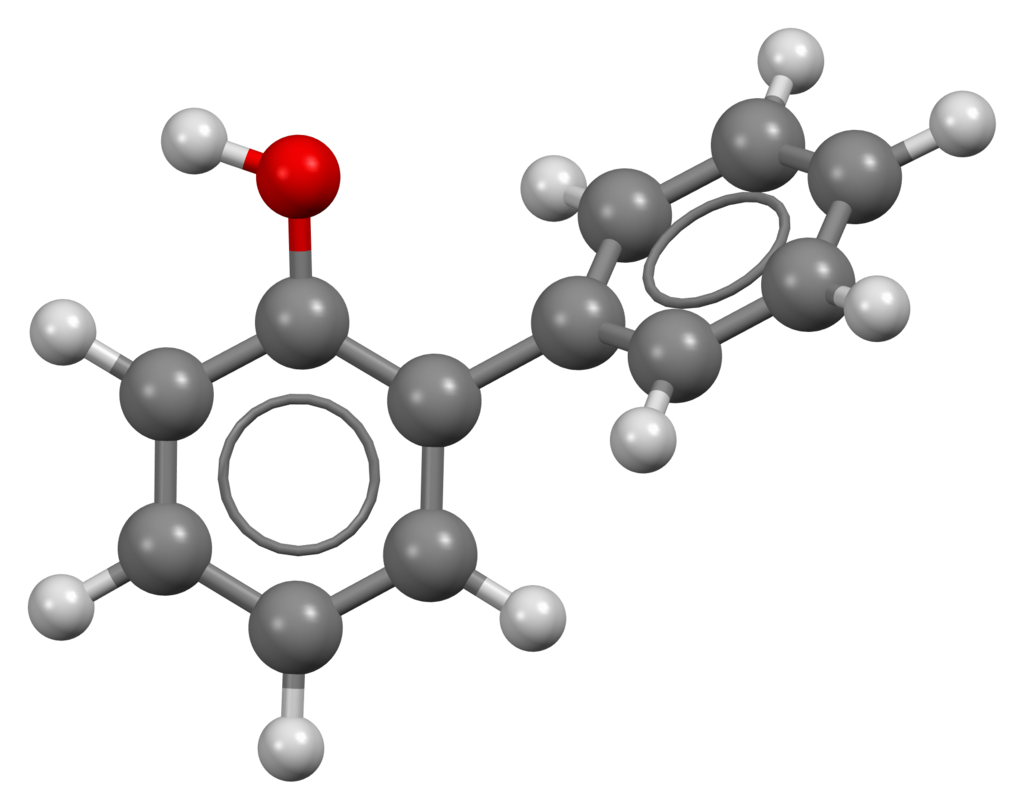
\includegraphics{p2.png}}\\
Fig. 5. Input structure of 2-Phenylphenol
\end{center}
Slightly larger molecule to test the performance of the algorithm.
\end{frame}

\begin{frame}
\frametitle{Results}
\framesubtitle{$C_{12} H_{10} O$}
Simulation with 1000 walkers for 2000 time steps
\begin{center}
\scalebox{0.25}{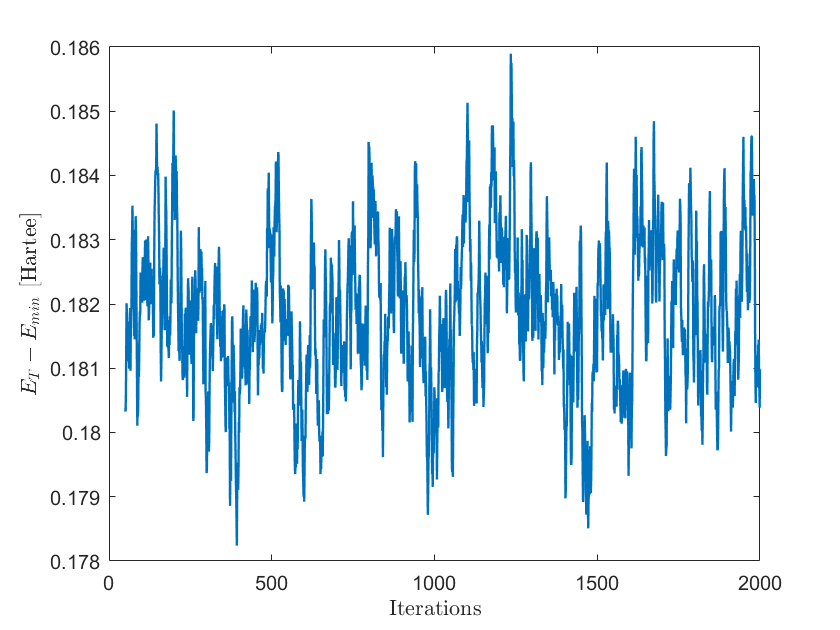
\includegraphics{fig3.png}}\\
Fig. 6. Fluctuation of the ZPE after equilibration.
\end{center}
ZPE = 0.18184 hartee with a standard deviation of 0.00117 hartee.\\


\end{frame}

\begin{frame}
\frametitle{Results}
\framesubtitle{$C_{12} H_{10} O$}
Simulation with 1000 walkers for 2000 time steps
\begin{center}
\scalebox{0.25}{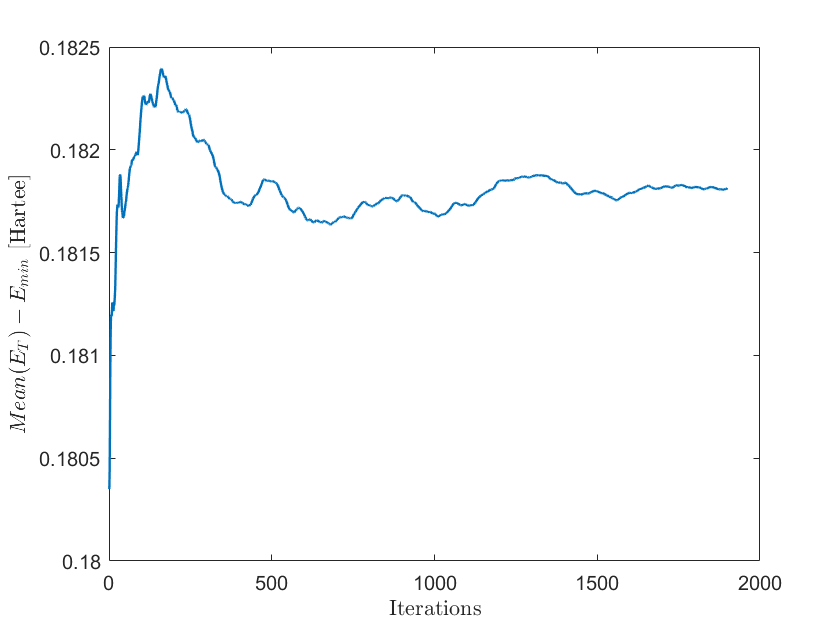
\includegraphics{fig4.png}}\\
Fig. 7. Convergence of the ZPE after equilibration.
\end{center}
Simulation time: 57 hours. $\approx$ 0.11 seconds per energy calculation.


\end{frame}

\subsection{$H_2@C_{60}$}

\begin{frame}
\frametitle{Results}
\framesubtitle{$H_2@C_{60}$}
\begin{center}
\scalebox{0.20}{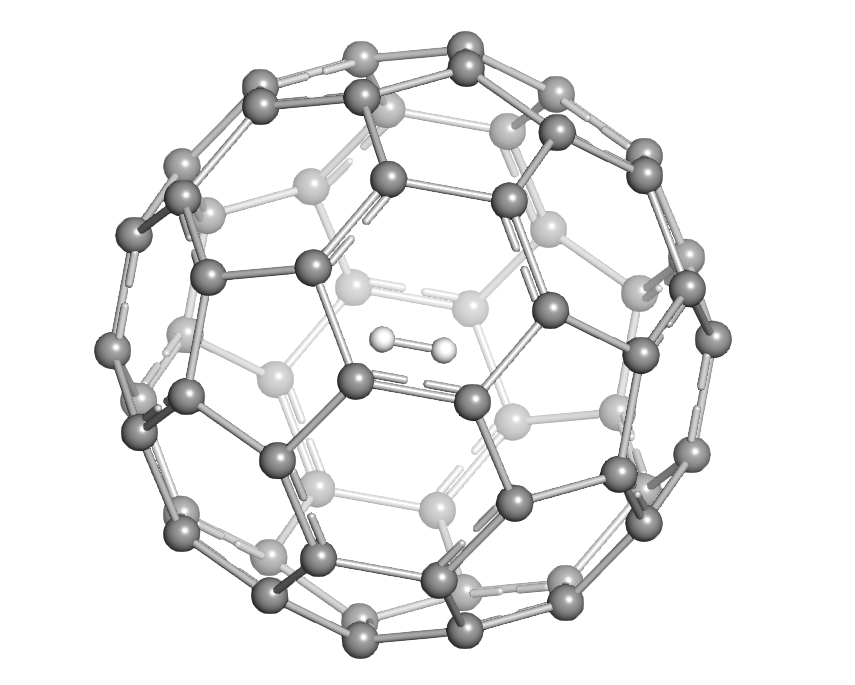
\includegraphics{p3.png}}\\
Fig. 8. Input structure of the dihydrogen endofullerene
\end{center}
The dihydrogen endofullerene is expected to show strong anharmonic effects on the zero point energy.\\
\end{frame}

\begin{frame}
\frametitle{Results}
\framesubtitle{$H_2@C_{60}$}
Simulation with 1000 walkers for 2000 time steps
\begin{center}
\scalebox{0.25}{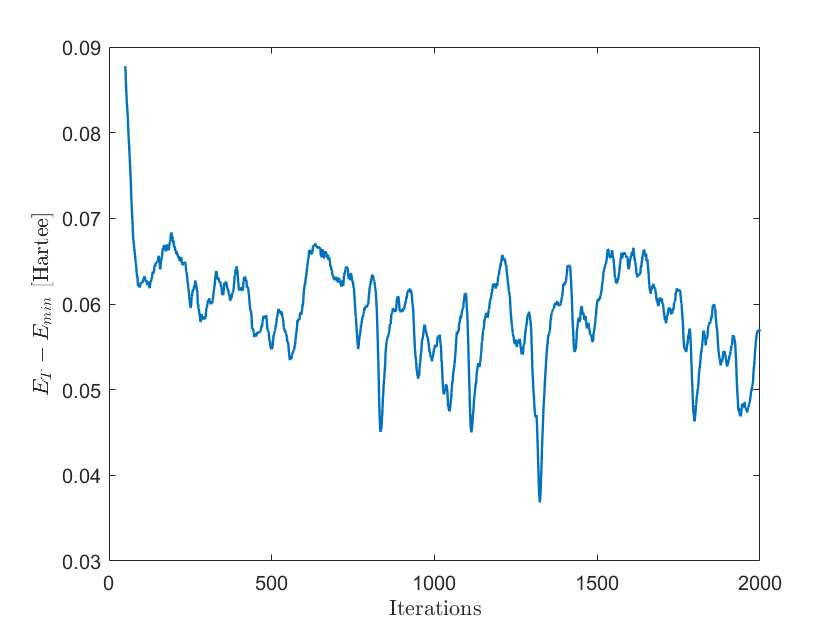
\includegraphics{fig5.png}}\\
Fig. 9. Fluctuation of the ZPE after equilibration.
\end{center}
ZPE = 0.05914 hartee with a standard deviation of 0.00569 hartee.\\

\end{frame}

\begin{frame}
\frametitle{Results}
\framesubtitle{$H_2@C_{60}$}
Simulation with 1000 walkers for 2000 time steps
\begin{center}
\scalebox{0.25}{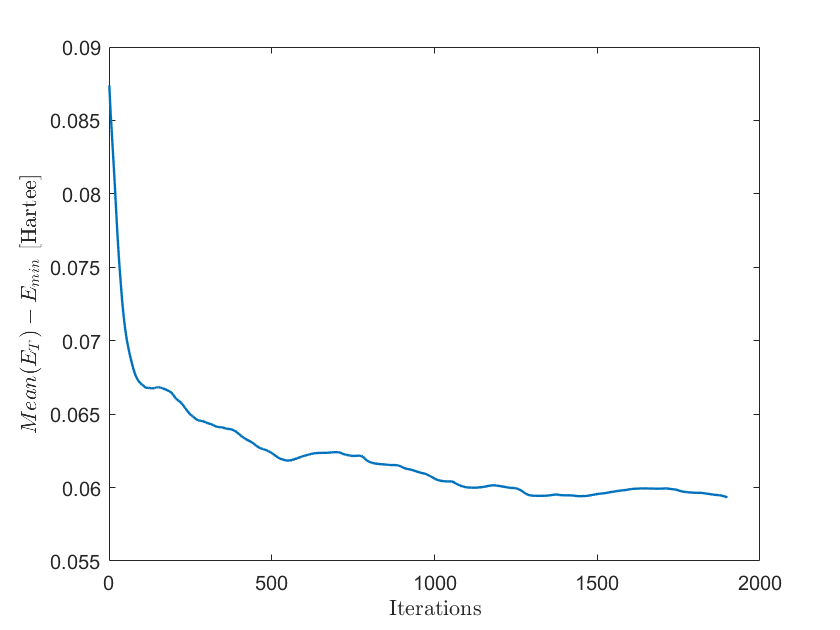
\includegraphics{fig6.png}}\\
Fig. 10. Convergence of the ZPE after equilibration.
\end{center}
Simulation time: 51 hours. $\approx$ 0.10 seconds per energy calculation.
\end{frame}

\section{Conclusions and Improvements}
\begin{frame}
\frametitle{Conclusions and Improvements}
Conclusions:
\begin{itemize}
\item DQMC delivers moderately accurate results for the ZPE in reasonable time.
\item DQMC is very versatile and can calculate the ZPE of most molecules.
\end{itemize}
Improvements:
\begin{itemize}
\item Adjustments for periodic structures
\item Parallelization
\item Making it more user-friendly
\end{itemize}
\end{frame}


\begin{frame}
\frametitle{References}
\bibliographystyle{unsrt}
\begin{scriptsize}
\bibliography{references}
\end{scriptsize}
\end{frame}

\end{document}